\documentclass{article}
\usepackage{graphicx}
\usepackage{subfigure}
\usepackage{multicol}
\usepackage{multirow}
\usepackage{float}

\begin{document}
	\begin{figure}
		\centering
		\subfigure[Saksham 1]{
			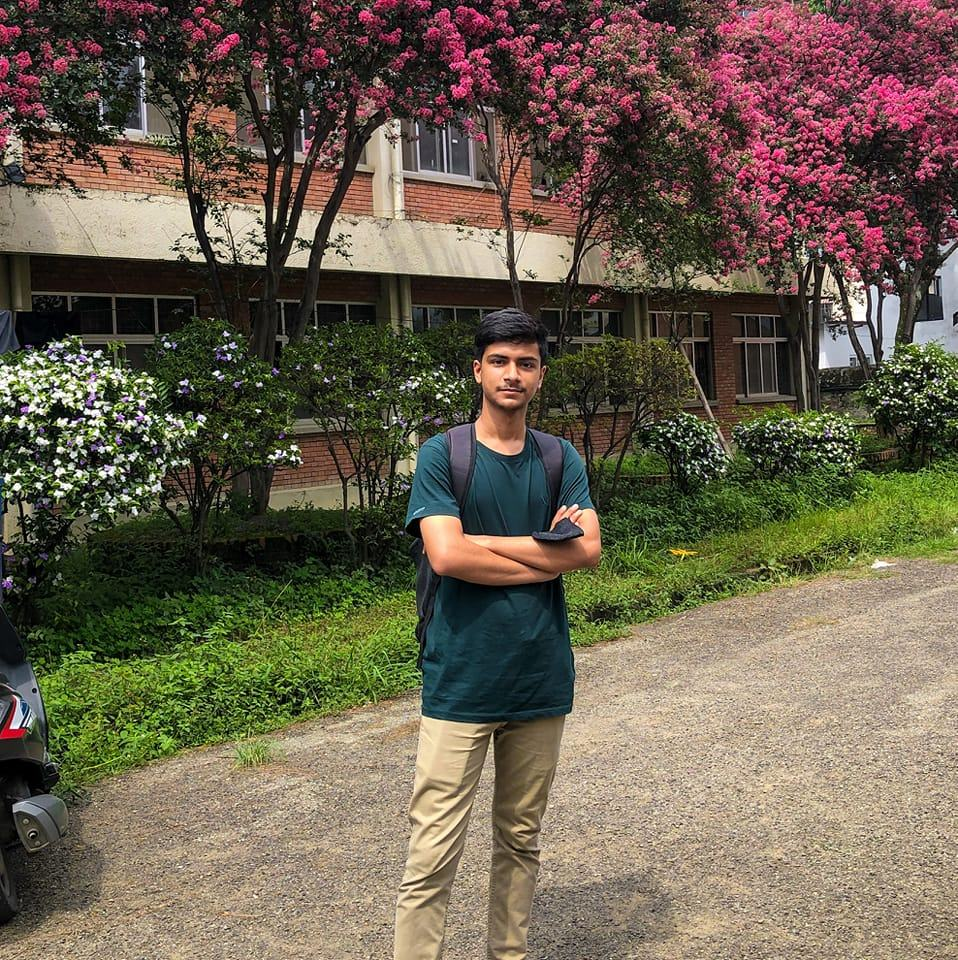
\includegraphics[width=1.5in]{C:/Users/jrsak/OneDrive/Pictures/img}
		}
		\subfigure[Saksham 2]{
			\includegraphics[width = 1.5in]{C:/Users/jrsak/OneDrive/Pictures/f.png}
		}
		\subfigure[Saksham 3]{
			\includegraphics[width = 1.5in]{C:/Users/jrsak/OneDrive/Pictures/IMG_5451.JPG}
		}
	\caption{Saksham}
	\end{figure}
	\centering
	\begin{tabular}{|l|c|c|}
		\hline
		\multicolumn{3}{|c|}{Students}\\\hline
		Name & Roll No. & Batch\\\hline
		Saksham Sapkota & 72 & 078 \\\hline
		Kripa Giri & 10 & 
		\multirow{2}{*}{079}\\\cline{1-2}
		Prajit Thapa & 40 & \\\hline
	\end{tabular}
\end{document}